% Chapter 2

\chapter{Literature Review} % Introduction

\label{Chapter2} % 

Within literature the most common way of tackling the problem is through Point Processes. More recently both Gaussian Processes and Deep Learning have been applied.

\section{Point Processes}
A temporal point process is a sequence of events ${t_i}$ with $t$ being a sequence of a fixed period inteveral with $t_i \epsilon R + and i \epsilon Z+$. It can be modelled as a series of inter-event times (time until next event) or the number of events occurring in the interval. Examples of point processes are the occurence of natural disasters, machine failure, or when a customer engages with a company.

At its simplest a point process can be represented as:
$${\xi =\sum _{i=1}^{n}\delta _{X_{i}},}$$

where $\delta$ denotes the Dirac measure, a probability measure of whether a set contains point x or not.

Point processes seek to model the probability of an event happening at time t, based on the event history upto, but not including, time t. Each point can either be seen as i.i.d. or as with the Wold process, dependent on the previouse inter-event time.
There are different ways of representing point process data as shown in figure \ref{fig:fig1}, with the inter-event time being the most common. In this form, the Poisson distribution is the most obvious choice for a conditional intensity function.

\begin{figure}[h!]
	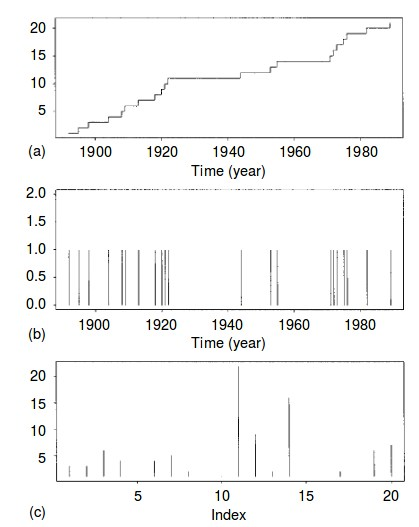
\includegraphics[width=7cm, keepaspectratio]{fig001.jpg}
	\caption{Three different representations of the same point-process a) cumulative count b) date of occurence c) interval time between floods}
	\label{fig:fig1}
\end{figure}

\textbf{Conditional Intensity Function} 

A condtional intensity function $\lambda(t)$ based on parametric statistics, such as a Poisson process for inter-event times, is used to determine the probability. 

\par
\textbf{Expectation measure} 

The expectation measure $E$ for a point process $\xi$ is the number of events p expected for every Borel subset of the event space S.

$$E\xi (B):=E{\bigl (}\xi (B){\bigr )}\quad {\text{for every }}B\in {\mathcal  {B}}$$

\section{Gaussian Processes}


\section{Deep Learning}

How it's referred to in lit:
* Event sequences

Methods:

Process Models
Temporal Points Processes
The point process representation of sequence data is
fundamentally different from the discrete time representation typically used in time series analysis. It
directly models the time period between events as random variables, and allows temporal events to
be modeled accurately, without requiring the choice of a time window to aggregate events, which
may cause discretization errors. Moreover, it has a remarkably extensive theoretical foundation [6].
However, conventional point process models often make strong unrealistic assumptions about the
generative processes of the event sequences. In fact, a point process is characterized by its conditional
intensity function – a stochastic model for the time of the next event given all the times of previous
events. The functional form of the intensity is often designed to capture the phenomena of interests.
Some examples are homogeneous and non-homogeneous Poisson processes [7], self-exciting point
processes [8], self-correcting point process models [9], and survival processes [6]. Unfortunately,they make various parametric assumptions about the latent dynamics governing the generation of the
observed point patterns. As a consequence, model misspecification can cause significantly degraded
performance using point process models, which is also shown by our experimental results later.

To address the aforementioned problem, the authors in [10] propose to learn a general representation
of the underlying dynamics from the event history without assuming a fixed parametric form in
advance. The intensity function of the temporal point process is viewed as a nonlinear function of
the history of the process and is parameterized using a recurrent neural network. Apparently this
line of work still relies on explicit modeling of the intensity function. However, in many tasks such
as data generation or event prediction, knowledge of the whole intensity function is unnecessary. we are able to demonstrate that Wasserstein distance training of RNN point
process models outperforms the same architecture trained using MLE.i) We propose the first intensity-free generative model
for point processes and introduce the first (to our best knowledge) likelihood-free corresponding
learning methods; ii)-3mm We extend WGAN for point processes with Recurrent Neural Network
architecture for sequence generation learning; iii) In contrast to the usual subjective measures of
evaluating GANs we use a statistical and a quantitative measure to compare the performance of the
model to the conventional ones. iv) Extensive experiments involving various types of point processes
on both synthetic and real datasets show the promising performance of our approach.
(Wasserstein Learning of Deep Generative Point)

